\begin{figure}
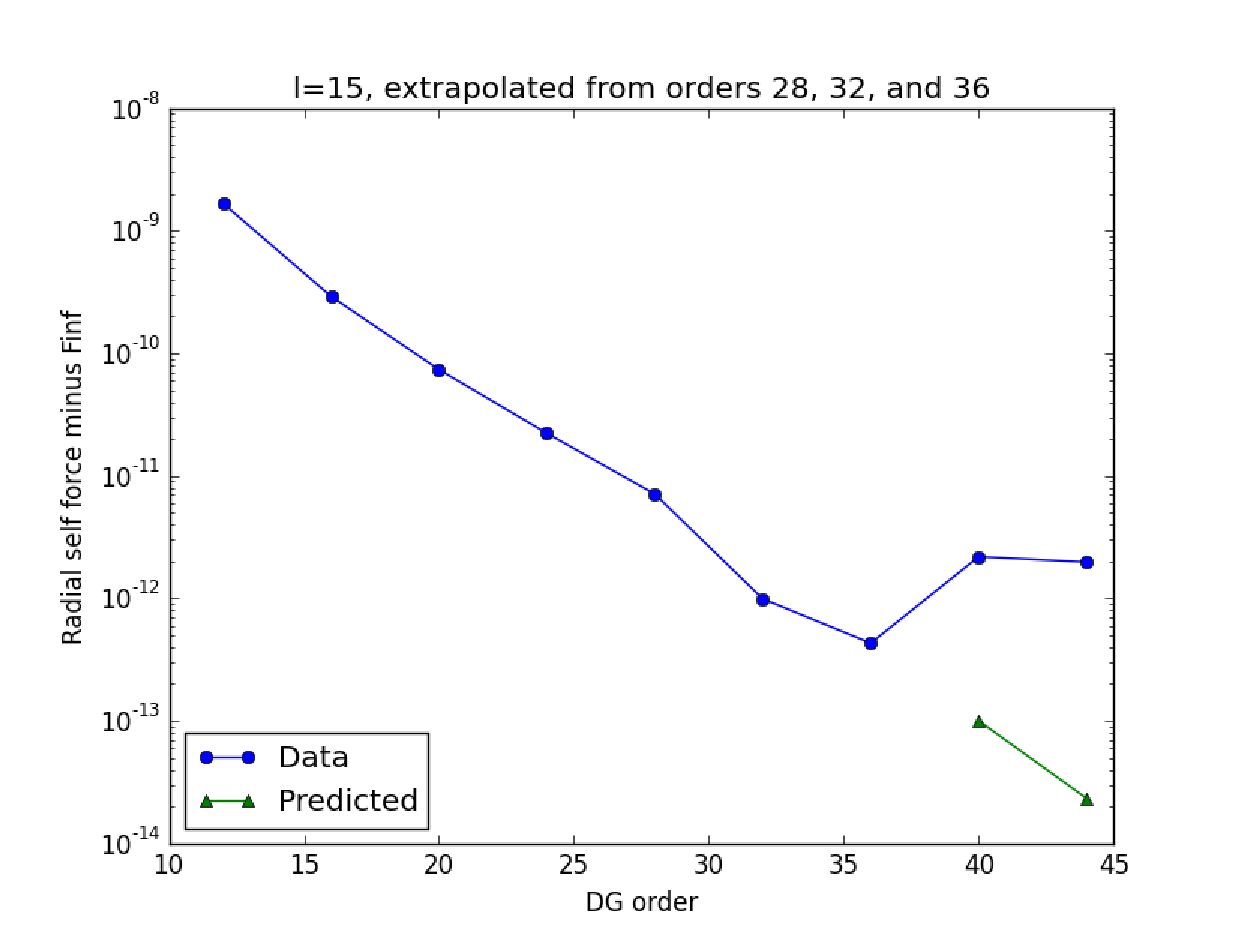
\includegraphics{/home/sdorsher/LabNotebook/20170713/extrapolate7plot}
\end{figure}

\begin{figure}
  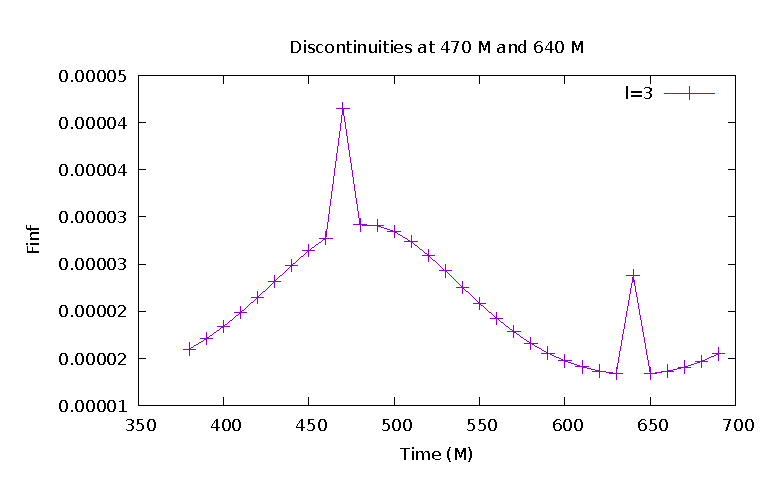
\includegraphics{/home/sdorsher/LabNotebook/20170714/finfovertimel3discontinuities}
\end{figure}




t472
\begin{table}
\begin{tabular}{ll}
Starting index & finf\\
2 & 4.18128309016e-05\\
3 & mode failed\\
4 & 4.18128307505e-05\\
5 & 4.18128308245e-05\\
6 & 4.1812830828e-05\\
\end{tabular}
\end{table}


\begin{figure}
  \includegraphics{/home/sdorsher/LabNotebook/20170719/extrapolate7t472l3i2}
\end{figure}

\begin{figure}
  \includegraphics{/home/sdorsher/LabNotebook/20170719/extrapolate7t472l2i3}
  \caption{Note that the three points used in the extrapolation are not on a line on a semilog scale-- it is not possible to fit an exponential through them. That is why this mode failed.}
\end{figure}

\begin{figure}
  \includegraphics{/home/sdorsher/LabNotebook/20170719/extrapolate7lt472l2i5}
\end{figure}

\begin{figure}
  \includegraphics{/home/sdorsher/LabNotebook/20170719/extrapolate7t472l2i6}
\end{figure}

\begin{figure}
  \includegraphics{/home/sdorsher/LabNotebook/20170719/manuallyChosenBestFinft472}
\end{figure}


\section{l=2}
\begin{table}
  \begin{tabular}{lll}
    time & starting order & finf\\
    632 & 0 & mode failed\\
    632 & 1 & 2.40975299617e-05\\
    632 & 2 & 2.40975300465e-05\\
    632 & 3 & 2.40975300114e-05\\
    632 & 4 & mode failed\\
    632 & 5 & 2.40975299291e-05\\
    632 & 6 & 2.40975299148e-05\\
    \hline
    634 & 0 & mode failed (however, 6 selected)\\
    634 & 1 & 2.39990698129e-05\\
    634 & 2 & 2.39990699318e-05\\
    634 & 3 & 2.39990698774e-05\\
    634 & 4 & mode failed\\
    634 & 5 & 2.39990697065e-05\\
    634 & 6 & 2.39990696758e-05\\
    \hline
    636 & 0 & mode failed (however, 6 selected)\\
    636 & 1 & 2.391047416e-05\\
    636 & 2 & 2.39104742806e-05\\
    636 & 3 & 2.39104742249e-05\\
    636 & 4 & 2.39104737911e-05\\
    636 & 5 & 2.39104739924e-05\\
    636 & 6 & 2.39104739079e-05\\
  \end{tabular}
\end{table}

\begin{figure}
  \includegraphics{/home/sdorsher/LabNotebook/20170720/extrapolate7t632l2i1}
\end{figure}

\begin{figure}
  \includegraphics{/home/sdorsher/LabNotebook/20170720/extrapolate7t632l2i2}
\end{figure}

\begin{figure}
  \includegraphics{/home/sdorsher/LabNotebook/20170720/extrapolate7t632l2i3}
\end{figure}

\begin{figure}
  \includegraphics{/home/sdorsher/LabNotebook/20170720/extrapolate7t632l2i5}
\end{figure}

\begin{figure}
  \includegraphics{/home/sdorsher/LabNotebook/20170720/extrapolate7t634l2i6}
\end{figure}

\begin{figure}
  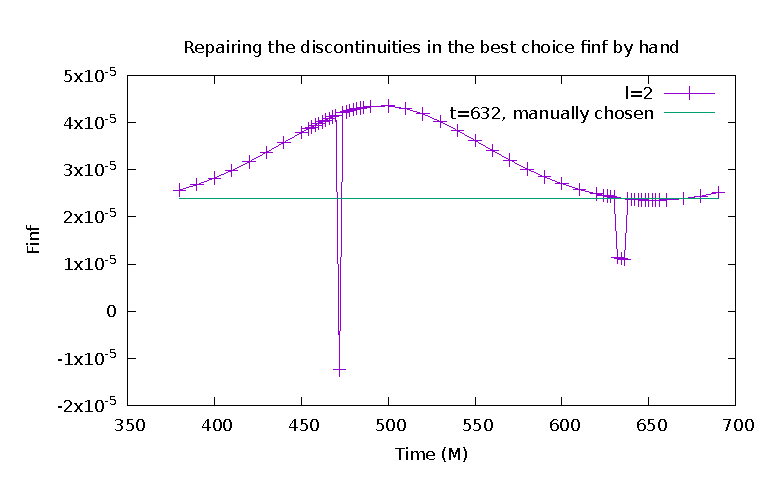
\includegraphics{/home/sdorsher/LabNotebook/20170720/bestFinfManuallyChosent632l2}
\end{figure}

\subsection{ Checking for discontinuities in $F_{\inf}$ for each each l-mode}

There are no discontinuities in $F_{\inf}$ for any of the l-modes when the median approach is used. See mode zero for an example.

\begin{figure}
  \includegraphics{/home/sdorsher/LabNotebook/20170727/finfovertimel0}
  \caption{An example of no discontinuities in $F_{\inf}$ for any of the l-modes. Mode $l=0$.}
\end{figure}


\subsection{Determining $F_{\inf}$ using maximum likelihood fits to subsegments of lines in semilog space}
Fit subsegments of lines in semilog space on DG order convergence plot after subtracting Finf for each possible starting order. pick starting order and starting and ending index of line segment with best possible chi-sq per dof (closest to one). use that finf. veto modes and starting indices that fail the alpha ratio test.

take standard deviation of surface plot as well as average.
\begin{figure}
  \includegraphics{fittingtechniqet370l0}
  \caption{l=0 mode with fit-chosen starting index produces convergence plot with nice long exponentially converging region}
\end{figure}





